%=============================================================================
% chktex-file 1 chktex-file 8 chktex-file 12 chktex-file 13 chktex-file 24 chktex-file 26
% CHAPITRE 2 : SPÉCIFICATION ET ANALYSE DES BESOINS
%=============================================================================

\chapter{Spécification et Analyse des Besoins}
\label{chap:besoins}

\section{Introduction}

L'analyse des besoins s'appuie sur l'étude approfondie du processus de recouvrement dans le secteur du crédit-bail financier. Ce chapitre se décompose en plusieurs sections fondamentales : la définition du langage de modélisation et de la méthodologie adoptée, la spécification détaillée des exigences fonctionnelles et non fonctionnelles, l'analyse par la modélisation UML (diagrammes de cas d'utilisation par module et diagramme de classes), la planification des sprints, et enfin la présentation des architectures logique et physique du système ainsi que l'étude des outils technologiques.

\section{Langage de Modélisation et Méthodologie}

\subsection{Langage de Modélisation : UML}

Le langage \textbf{UML} (\textit{Unified Modeling Language}) est utilisé comme méthode standardisée de modélisation et de visualisation. Il facilite la conception orientée objet en décrivant formellement les interactions dynamiques du système (diagramme de cas d'utilisation) et sa structure statique (diagramme de classes).

\subsection{Méthodologie Adoptée : Scrum}

Pour mener à bien la conception et le développement de la plateforme \projectShortTitle, le framework Agile \textbf{Scrum} a été retenu. Il permet une livraison itérative et incrémentale. Face à la complexité d'une architecture multi-tenant et d'un pipeline d'intelligence artificielle, Scrum offre une transparence et une visibilité accrues sur l'avancement. Des sprints réguliers permettent de valider les fonctionnalités critiques telles que l'isolation des données ou l'extraction documentaire, tout en s'adaptant continuellement aux retours et aux enjeux d'intégration.

\section{Spécification des Besoins}

\subsection{Identification des Acteurs}

Le système interagit avec plusieurs acteurs présentant des responsabilités fonctionnelles distinctes :
\begin{itemize}
    \item \textbf{Super Admin (Éditeur LeasRecover) :} Crée, configure et supervise les \textit{tenants} (sociétés de leasing clientes). Il n'a aucun accès aux données contenues dans les dossiers clients de ses locataires.
    \item \textbf{Admin (Société cliente) :} Configure l'environnement spécifique à son tenant (image de marque, délais légaux par phase, seuils d'alerte IA) et gère les comptes de ses Gestionnaires.
    \item \textbf{Gestionnaire de Recouvrement :} Utilisateur opérationnel final. Il crée les dossiers, pilote le workflow en 5 phases, téléverse les rapports d'expertise et prend les décisions d'arbitrage de vente.
    \item \textbf{Module IA (Acteur Système) :} Composant automatisé qui analyse les rapports d'expertise de manière asynchrone, extrait les valeurs financières clés et calcule l'écart avec la valeur résiduelle initiale.
\end{itemize}

\subsection{Besoins Fonctionnels}

Les fonctionnalités attendues sont organisées en trois modules logiques principaux :

\subsubsection{Module 1 : Administration et Gestion des Tenants}
\begin{itemize}
    \item Création, activation, suspension et isolation stricte des tenants (sociétés de leasing).
    \item Configuration personnalisée des délais légaux par phase et des seuils d'inactivité/dormance.
    \item Gestion granulaire des utilisateurs et des permissions associées aux rôles au sein du tenant.
\end{itemize}

\subsubsection{Module 2 : Cœur Métier (Dossiers et Workflow)}
\begin{itemize}
    \item Création et suivi des dossiers de recouvrement rattachés à un client débiteur, un contrat de leasing et un véhicule.
    \item Progression conditionnelle via 5 phases séquentielles : \textbf{Pré-contentieux} $\rightarrow$ \textbf{Mise en demeure} $\rightarrow$ \textbf{Saisie} $\rightarrow$ \textbf{Vente} $\rightarrow$ \textbf{Clôture}.
    \item Génération automatique d'alertes à l'approche de l'expiration d'un délai légal ou d'un seuil d'inactivité critique.
    \item Coffre-fort documentaire sécurisé pour le stockage des pièces juridiques.
\end{itemize}

\subsubsection{Module 3 : Intelligence Artificielle et Évaluation Documentaire}
\begin{itemize}
    \item Téléversement sécurisé de rapports d'expertise PDF et déclenchement automatique du pipeline asynchrone IA.
    \item Extraction sémantique de la valeur marchande ($\ve$) et confrontation instantanée à la valeur résiduelle contractuelle ($\vr$).
    \item Génération d'un indicateur de fiabilité financière explicite (\textit{Fiable}, \textit{Écart modéré}, \textit{Écart critique}).
\end{itemize}

\subsection{Besoins Non Fonctionnels}

Les exigences non fonctionnelles garantissent la robustesse et l'opérabilité de la plateforme B2B :
\begin{itemize}
    \item \textbf{Performance :} Le pipeline IA complet doit s'exécuter en moins de 30 secondes par rapport d'expertise. Le tableau de bord principal doit se charger en moins de 2 secondes.
    \item \textbf{Sécurité et Confidentialité :} Chiffrement de niveau industriel (AES-256 au repos, TLS 1.2+ en transit) et isolation multi-tenant à tolérance zéro assurée au niveau de la base de données.
    \item \textbf{Traçabilité \& Conformité :} Enregistrement automatique de chaque action utilisateur dans un journal d'audit (\textit{Audit Trail}) immuable, garantissant la conformité avec le RGPD et la Loi n°63-2004.
    \item \textbf{Scalabilité \& Disponibilité :} Le microservice IA doit être déployé et mis à l'échelle indépendamment du reste de l'application métier.
\end{itemize}

\section{Analyse des Besoins}

\subsection{Diagrammes des Cas d'Utilisation}

Afin de garantir une lisibilité optimale et une modélisation rigoureuse des interactions, les cas d'utilisation de la plateforme \projectShortTitle{} sont découpés en quatre diagrammes modulaires correspondant aux grands packages fonctionnels et aux rôles des acteurs.

\subsubsection{Cas d'Utilisation 1 : Administration des Tenants et Politiques de Conformité}

Ce premier module (figure~\ref{fig:uc1_admin_compliance}) modélise l'espace d'administration de la plateforme, partagé entre le Super Administrateur (éditeur de la solution) et l'Administrateur de l'organisme de leasing :

\begin{figure}[H]
\centering
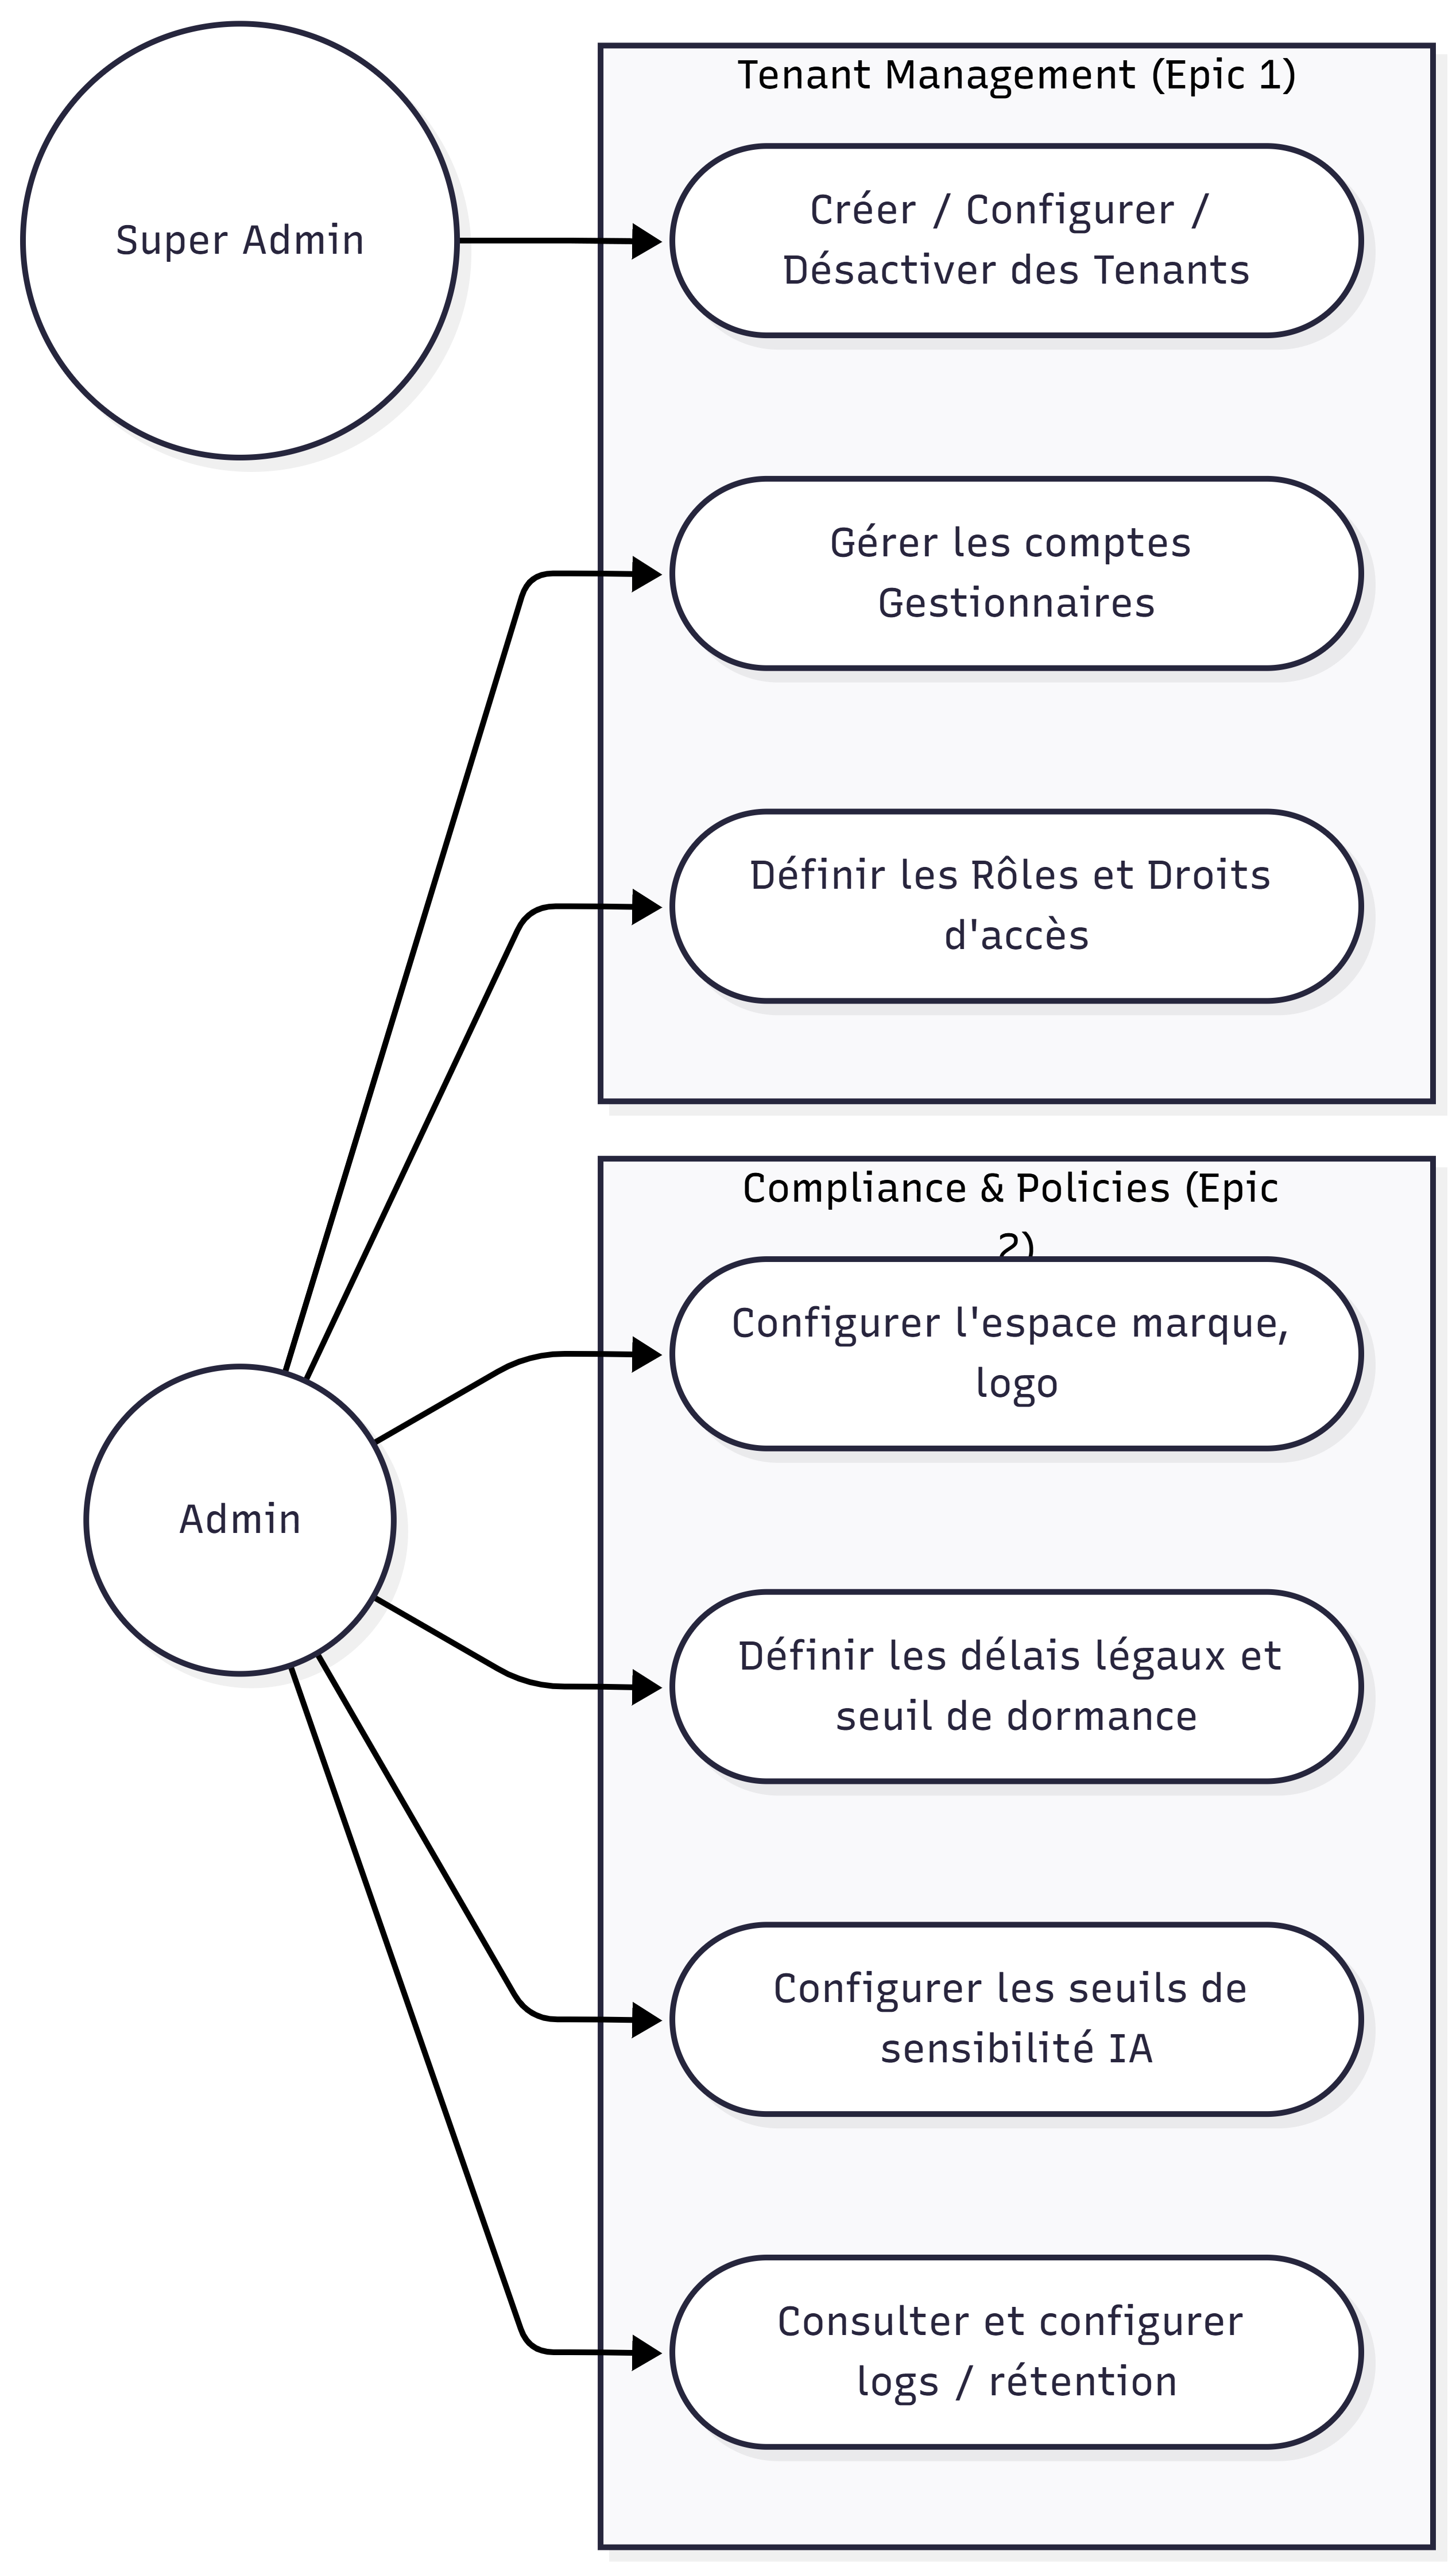
\includegraphics[width=\textwidth,height=0.62\textheight,keepaspectratio]{images/uc1.png}
\caption{Diagramme de cas d'utilisation -- Administration des Tenants et Conformité}
\label{fig:uc1_admin_compliance}
\end{figure}

\begin{itemize}
    \item \textbf{Super Administrateur (Éditeur LeasRecover) :}
    \begin{itemize}
        \item \textit{Créer, Configurer et Désactiver des Tenants :} Provisionnement sécurisé d'une nouvelle société cliente, instanciation automatique de son schéma de données étanche et gestion de l'état d'activité de l'instance.
    \end{itemize}
    \item \textbf{Administrateur (Société de leasing cliente) :}
    \begin{itemize}
        \item \textit{Gestion des comptes gestionnaires :} Création, affectation et révocation des accès des gestionnaires de recouvrement.
        \item \textit{Définition des rôles et privilèges :} Attribution granulaire des droits d'accès (RBAC) sur les dossiers et actions financières.
        \item \textit{Personnalisation de la marque (Tenant Branding) :} Téléversement du logo institutionnel et personnalisation visuelle de l'espace de travail.
        \item \textit{Paramétrage des délais légaux et seuil de dormance :} Définition des délais légaux maximaux par phase et du seuil d'inactivité déclenchant la qualification de dossier dormant.
        \item \textit{Configuration des seuils de sensibilité IA :} Définition des pourcentages d'écart de valeur déclenchant les alertes de dépréciation.
        \item \textit{Consultation des logs et politiques de rétention :} Traçabilité des actions administratives et configuration des durées de conservation des journaux d'audit.
    \end{itemize}
\end{itemize}

\subsubsection{Cas d'Utilisation 2 : Gestion des Référentiels Métiers et Dossiers de Recouvrement}

Le deuxième module (figure~\ref{fig:uc2_core_cases}) détaille la gestion du référentiel métier ainsi que le cycle de vie opérationnel des dossiers de recouvrement contentieux :

\begin{figure}[H]
\centering
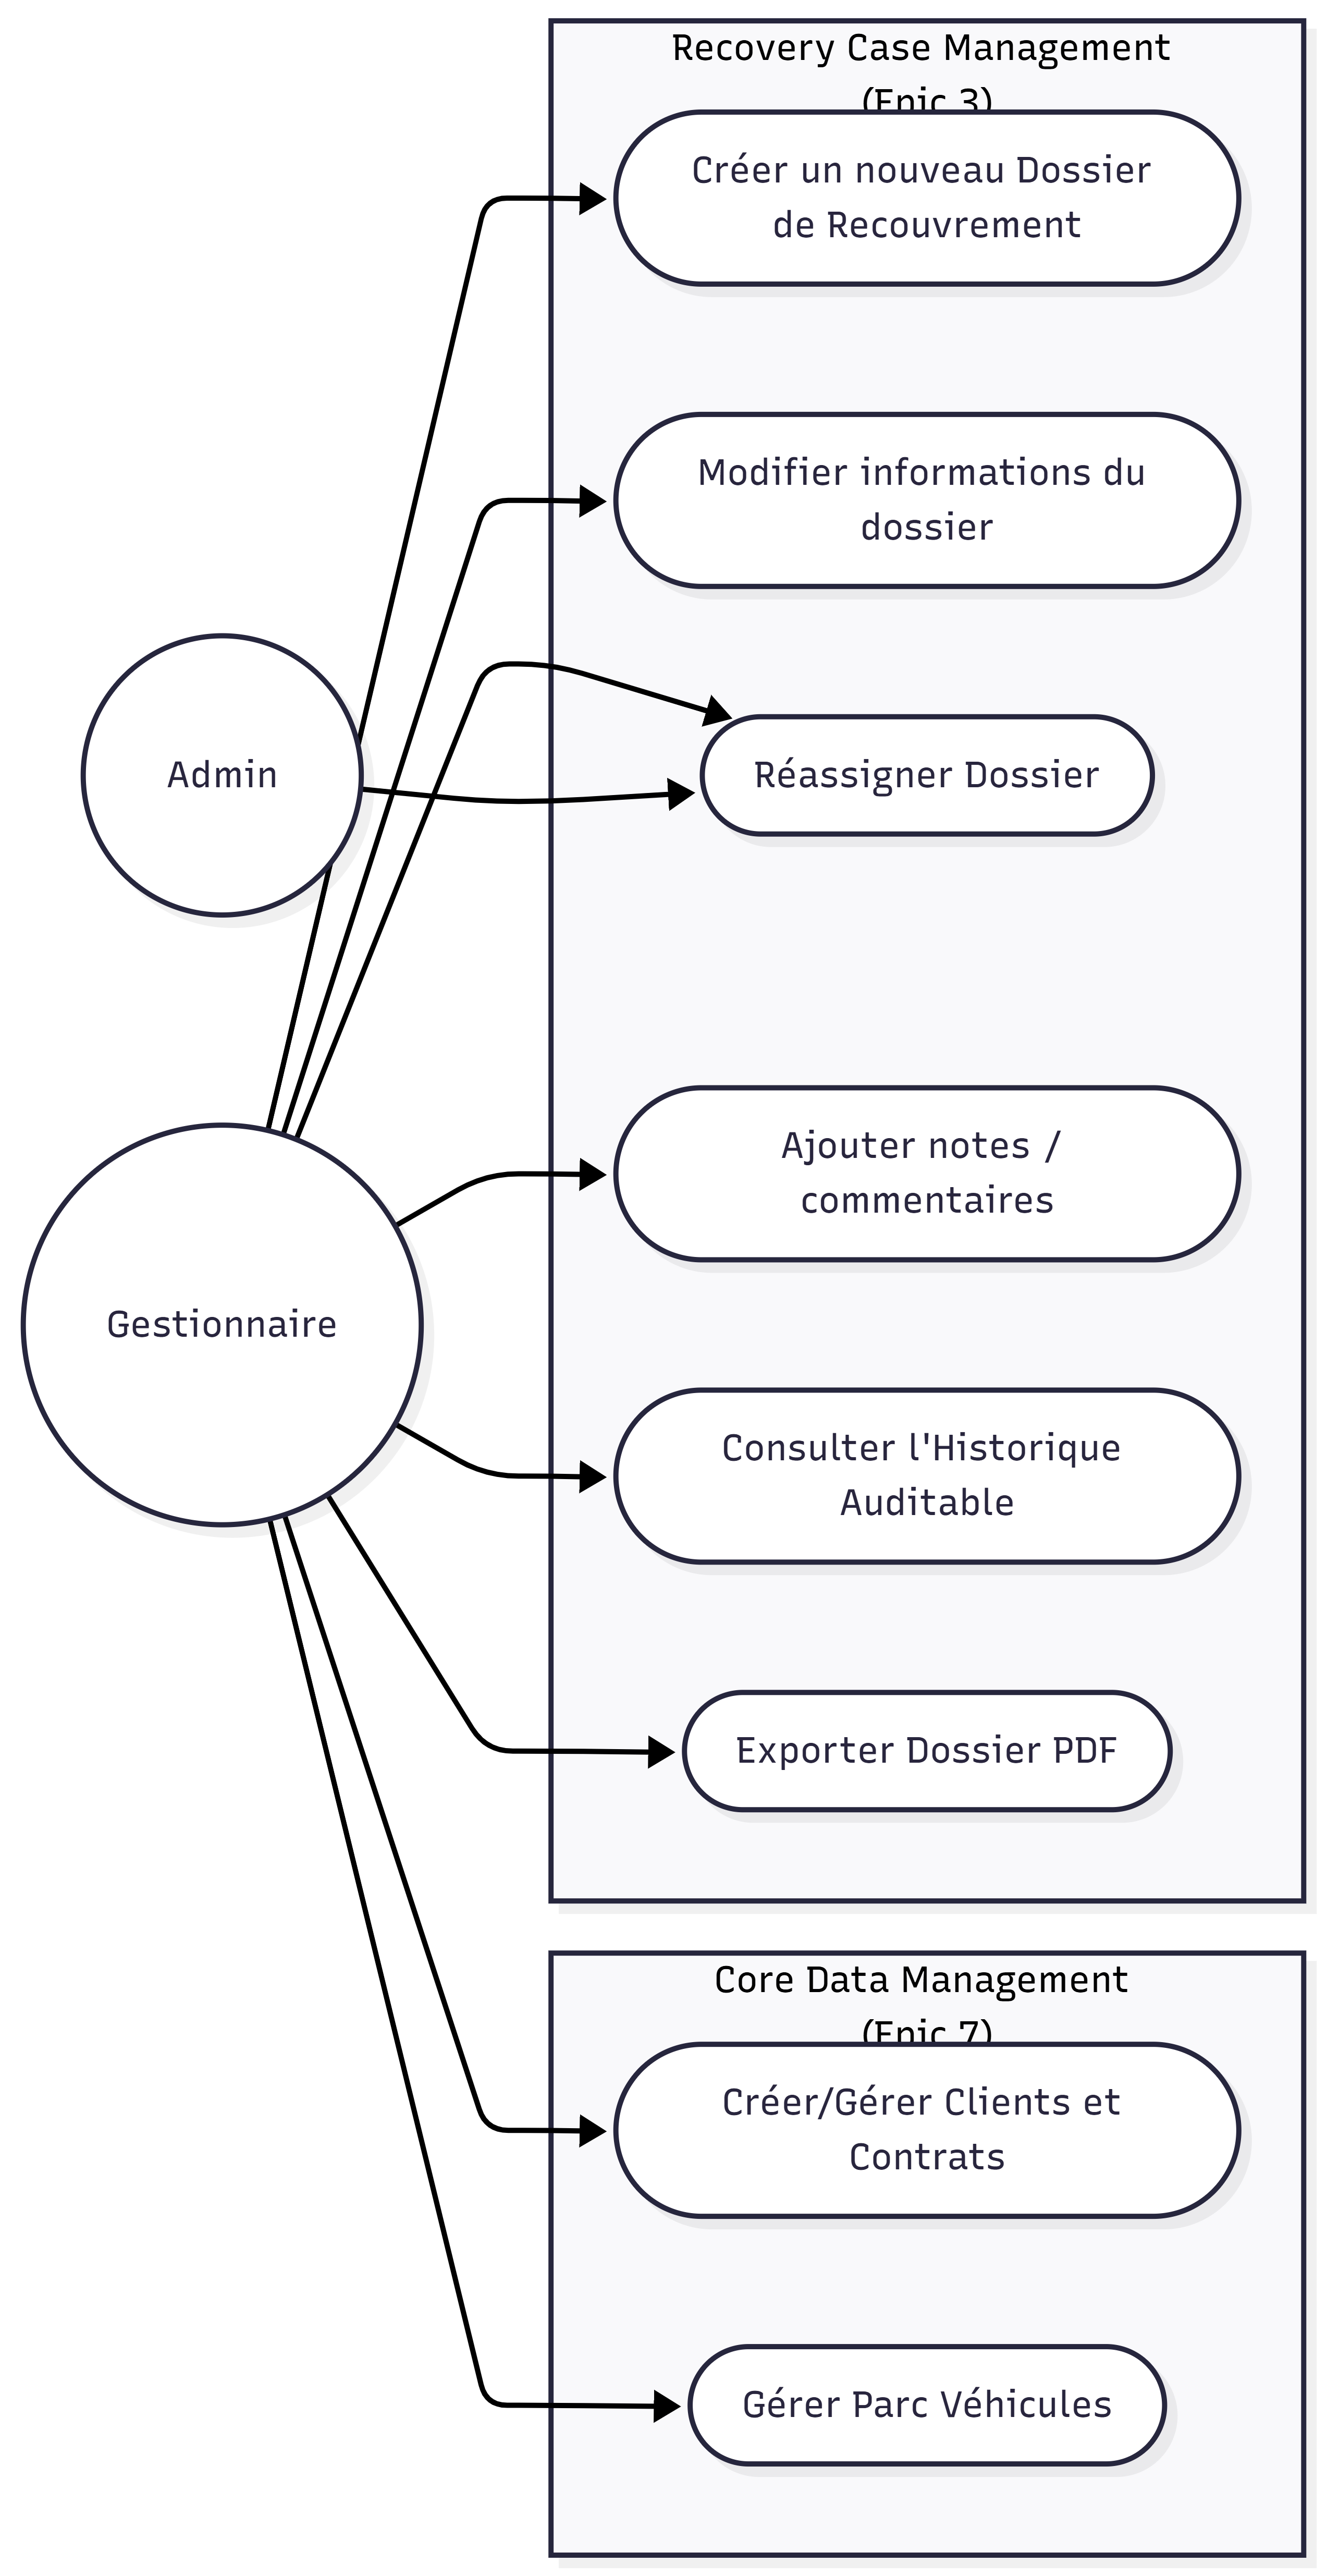
\includegraphics[width=\textwidth,height=0.62\textheight,keepaspectratio]{images/uc2.png}
\caption{Diagramme de cas d'utilisation -- Référentiels Métiers et Dossiers}
\label{fig:uc2_core_cases}
\end{figure}

\begin{itemize}
    \item \textbf{Gestion des Référentiels Métiers (Core Data) :}
    \begin{itemize}
        \item Le \textbf{Gestionnaire de Recouvrement} administre les fiches clients débiteurs (coordonnées, solvabilité), les contrats de crédit-bail associés (valeur résiduelle contractuelle $\vr$, montants impayés) ainsi que le parc de véhicules (numéro VIN, immatriculation, état).
    \end{itemize}
    \item \textbf{Gestion des Dossiers de Recouvrement (Recovery Case Management) :}
    \begin{itemize}
        \item \textit{Création et initialisation :} Ouverture d'un nouveau dossier suite au basculement d'un contrat en défaut de paiement.
        \item \textit{Mise à jour des informations :} Édition des métadonnées du dossier et consignation des événements d'instruction.
        \item \textit{Réassignation de dossier :} Possibilité pour l'\textbf{Administrateur} ou le Gestionnaire de réaffecter la charge d'un dossier à un collègue.
        \item \textit{Annotations et notes de suivi :} Ajout d'observations textuelles et de pièces horodatées.
        \item \textit{Consultation de l'historique et export PDF :} Visualisation de l'historique complet auditable et génération d'un rapport de synthèse imprimable.
    \end{itemize}
\end{itemize}

\clearpage
\subsubsection{Cas d'Utilisation 3 : Workflow Légal, Documents et Pipeline IA}

Le troisième module (figure~\ref{fig:uc3_workflow_ai}) illustre l'interaction entre le gestionnaire opérationnel et les processus automatisés du système et du service IA :

\begin{figure}[H]
\centering

\includegraphics[width=\textwidth,height=0.62\textheight,keepaspectratio]{images/uc3.png}
\caption{Diagramme de cas d'utilisation -- Workflow Légal, Documents et Pipeline IA}
\label{fig:uc3_workflow_ai}
\end{figure}

\begin{itemize}
    \item \textbf{Workflow Légal et Coffre-fort Documentaire :}
    \begin{itemize}
        \item \textit{Téléversement et consultation documentaire :} Le Gestionnaire dépose et archive les pièces probantes (mises en demeure, procès-verbaux d'huissier, rapports d'expertise).
        \item \textit{Progression des phases juridiques :} Le Gestionnaire initie le passage d'une phase à la suivante (\textbf{Pré-contentieux} $\rightarrow$ \textbf{Mise en demeure} $\rightarrow$ \textbf{Saisie} $\rightarrow$ \textbf{Vente} $\rightarrow$ \textbf{Clôture}).
        \item \textit{Contrôle automatisé des prérequis :} Le \textbf{Système} bloque dynamiquement la transition si les documents obligatoires ou les délais minimaux ne sont pas respectés.
        \item \textit{Surveillance des délais légaux :} Le Système émet des alertes proactives à l'approche de la date d'expiration légale d'une phase.
    \end{itemize}
    \item \textbf{Pipeline d'Évaluation Documentaire par Intelligence Artificielle :}
    \begin{itemize}
        \item \textit{Déclenchement du pipeline :} Déclenché manuellement par le Gestionnaire ou automatiquement par le Système lors du téléversement d'un rapport PDF.
        \item \textit{Extraction sémantique NLP/OCR :} Le microservice IA extrait la valeur vénale estimée ($\ve$), le kilométrage et l'état général de l'actif.
        \item \textit{Confrontation financière :} Le Système calcule automatiquement la déviation absolue ($\Delta = \ve - \vr$) et le ratio de couverture ($R$).
        \item \textit{Génération d'indicateur de fiabilité :} Attribution d'un statut décisionnel explicite (\textit{Fiable}, \textit{Écart modéré}, \textit{Écart critique}) guidant le choix d'arbitrage de vente.
    \end{itemize}
\end{itemize}

\clearpage
\subsubsection{Cas d'Utilisation 4 : Command Center, Sécurité et Traçabilité}

Le quatrième module (figure~\ref{fig:uc4_dashboard_security}) regroupe les fonctionnalités du poste de pilotage quotidien ainsi que les mécanismes transversaux de sécurité et d'audit :

\begin{figure}[H]
\centering
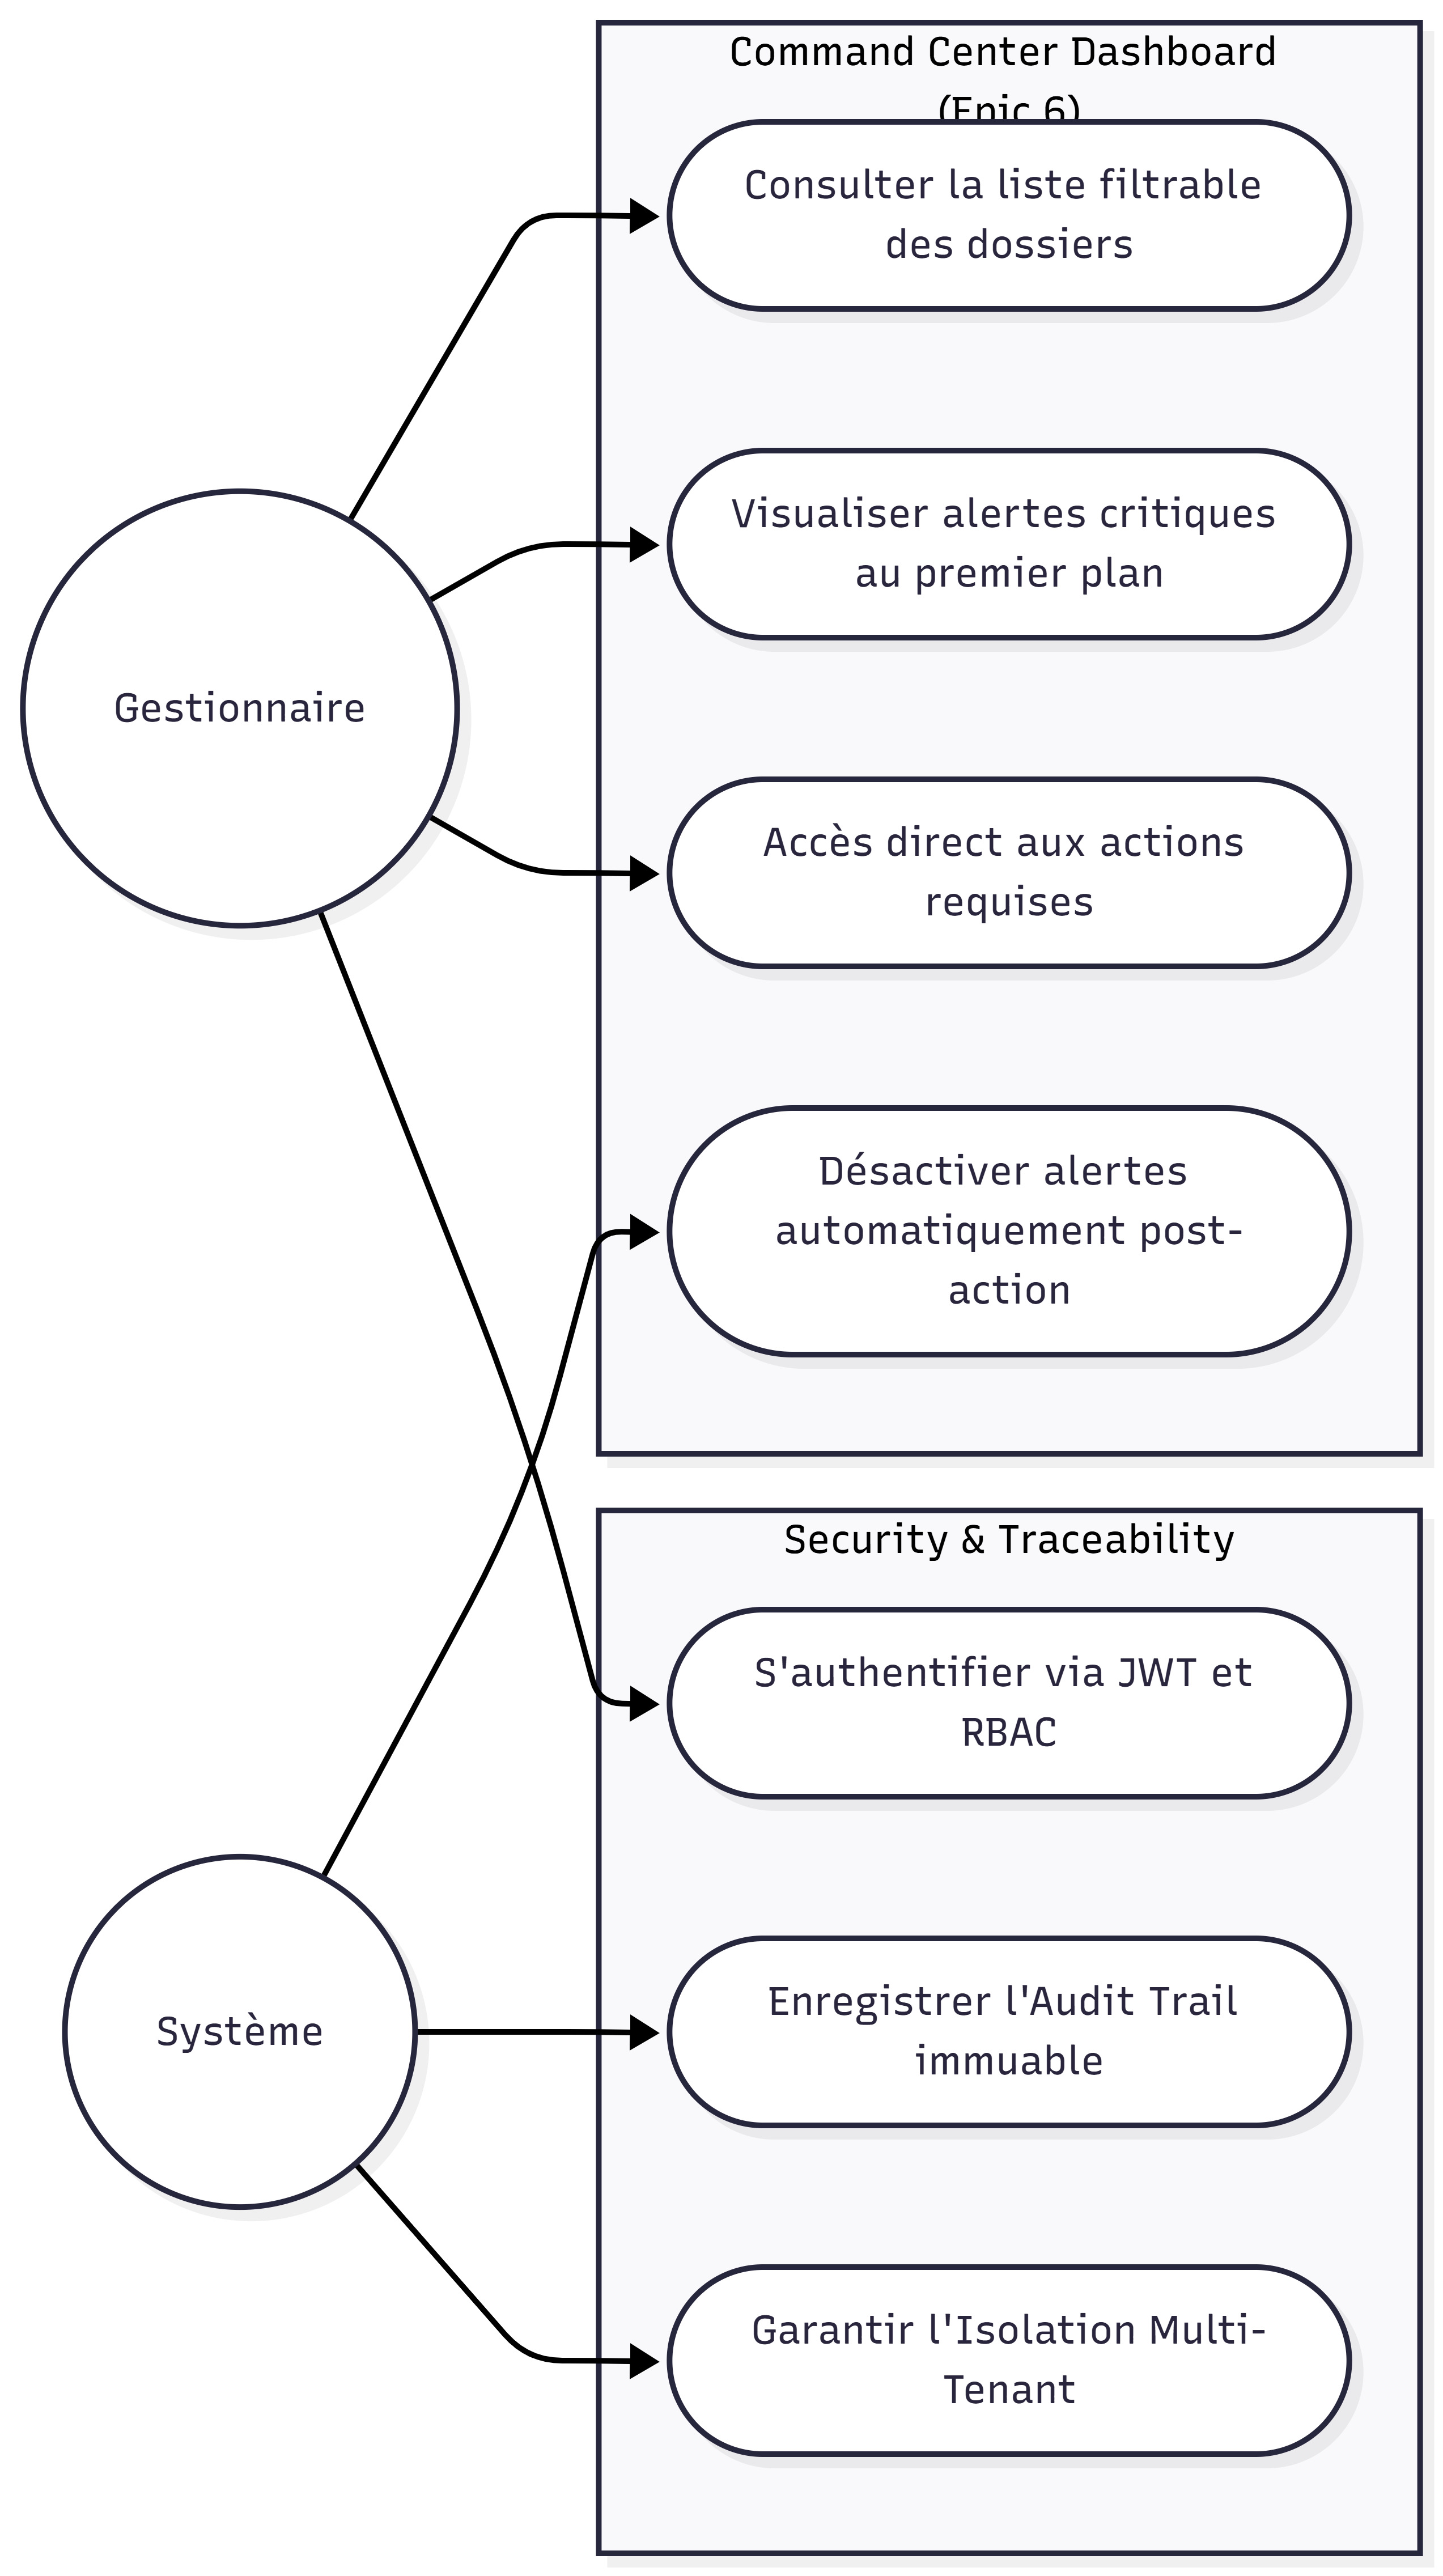
\includegraphics[width=\textwidth,height=0.62\textheight,keepaspectratio]{images/uc4.png}
\caption{Diagramme de cas d'utilisation -- Command Center, Sécurité et Traçabilité}
\label{fig:uc4_dashboard_security}
\end{figure}

\begin{itemize}
    \item \textbf{Tableau de Bord Opérationnel (Command Center Dashboard) :}
    \begin{itemize}
        \item \textit{Registre global filtrable :} Vue unifiée permettant au Gestionnaire de filtrer et trier les dossiers selon la phase, le niveau de criticité ou l'agent assigné.
        \item \textit{Visualisation des alertes critiques :} Mise en évidence des alertes d'expiration de délais légaux, d'anomalies financières IA ou de dormance.
        \item \textit{Accès direct aux actions prioritaires :} Liens d'action rapide permettant d'intervenir immédiatement sur le dossier concerné.
        \item \textit{Désactivation automatique post-action :} Le Système acquitte et clôture les alertes dès l'exécution de l'action corrective requise.
    \end{itemize}
    \item \textbf{Sécurité, Isolation et Traçabilité Système :}
    \begin{itemize}
        \item \textit{Authentification sécurisée et RBAC :} Gestion des sessions par cookies chiffrés et contrôle d'accès strict selon les rôles.
        \item \textit{Piste d'audit immuable (Audit Trail) :} Enregistrement systématique de toutes les créations, modifications et consultations dans un journal infalsifiable.
        \item \textit{Garantie de l'isolation multi-tenant :} Ségrégation stricte des données au niveau de la couche d'accès aux bases de données.
    \end{itemize}
\end{itemize}

\subsection{Diagramme de Classes du Système}

\begin{figure}[H]
\centering

\includegraphics[width=\textwidth,height=2\textheight,keepaspectratio]{images/class_diagram.png}
\caption{Diagramme de classes du système LeasRecover}
\label{fig:class_diagram}
\end{figure}

Le modèle conceptuel de classes (figure~\ref{fig:class_diagram}) respecte les principes d'isolation multi-tenant et de normalisation logicielle :
\begin{itemize}
    \item \textbf{BaseEntity \& TenantAwareEntity :} Classes de base gérant universellement les identifiants uniques (UUID v7), l'audit de création/modification et la clé étrangère \code{tenant_id} fondamentale pour l'étanchéité des données.
    \item \textbf{Entités Métiers :} Classes concrètes modélisant le domaine (\code{Tenant}, \code{User}, \code{RecoveryCase}, \code{Vehicle}, \code{Contract}, \code{AiValuation}, \code{AuditLog}).
\end{itemize}

\section{Planification du Projet}

\subsection{Backlog du Produit}

Le backlog produit a été décomposé en 7 Épiques (\textit{Epics}) fonctionnelles majeures :
\begin{itemize}
    \item \textbf{Epic 1 \& 2 :} Fondations Tenant, Identité et Configuration des politiques de conformité.
    \item \textbf{Epic 3 \& 4 :} Gestion cœur des dossiers, coffre-fort documentaire et respect du workflow légal.
    \item \textbf{Epic 5 \& 6 :} Pipeline d'évaluation intelligente (IA) et Tableau de bord (\textit{Command Center}).
    \item \textbf{Epic 7 :} Référentiels métiers (Clients, Contrats, Véhicules).
\end{itemize}

\clearpage
\subsection{Planification des Sprints et Livrables}

Le projet a été exécuté sur 8 sprints itératifs de deux à trois semaines, détaillés dans le tableau~\ref{tab:planification_sprints}.

\begin{table}[H]
\centering
\small
\caption{Planification des Sprints et Livrables du Projet LeasRecover}
\label{tab:planification_sprints}
\begin{tabularx}{\textwidth}{@{}L{2cm} L{2.2cm} L{6.2cm} Y@{}}
\toprule
\textbf{Sprint} & \textbf{Épique} & \textbf{Objectifs et User Stories} & \textbf{Livrable} \\
\midrule
\textbf{Sprint 1} & Epic 1 (Part. 1) & Initialisation du projet, schéma de base de données global et infrastructure multi-tenant (Stories 1.1, 1.2). & DB prête avec séparation stricte des tenants. \\
\addlinespace
\textbf{Sprint 2} & Epic 1 (Part. 2) & Gestion des utilisateurs, authentification sécurisée via BFF et gestion des sessions (Stories 1.3, 1.4). & Authentification opérationnelle. \\
\addlinespace
\textbf{Sprint 3} & Epic 2 & Politiques de conformité : image de marque, délais légaux, seuils IA (Stories 2.1 à 2.3). & Interface d'administration et règles configurables. \\
\addlinespace
\textbf{Sprint 4} & Epic 7 & Gestion des données de base : Clients, Contrats, Véhicules, documents (Stories 7.1 à 7.3). & Référentiels métiers fonctionnels. \\
\addlinespace
\textbf{Sprint 5} & Epic 3 & Cœur du système : Création/modification des dossiers, Audit Trail (Stories 3.1 à 3.4). & Gestion de l'historique et des dossiers. \\
\addlinespace
\textbf{Sprint 6} & Epic 4 & Workflow légal (5 phases), bloqueurs, alertes et coffre-fort documentaire (Stories 4.1 à 4.4). & Moteur de workflow et alertes de délais. \\
\addlinespace
\textbf{Sprint 7} & Epic 5 & Pipeline IA : Déclencheur API, extraction NLP, comparaison valeur/marché (Stories 5.1 à 5.5). & Module IA d'analyse intégré. \\
\addlinespace
\textbf{Sprint 8} & Epic 6 & Command Center : Registre dossiers, alertes critiques, actions rapides (Stories 6.1 à 6.4). & Tableau de pilotage finalisé. \\
\bottomrule
\end{tabularx}
\end{table}

\clearpage
\section{Architecture de la Solution}

\subsection{Architecture Logique du Système}

L'architecture logique de \projectShortTitle\ repose sur une approche modulaire découpée en trois couches indépendantes (figure~\ref{fig:logic_architecture}) :

\begin{figure}[H]
\centering
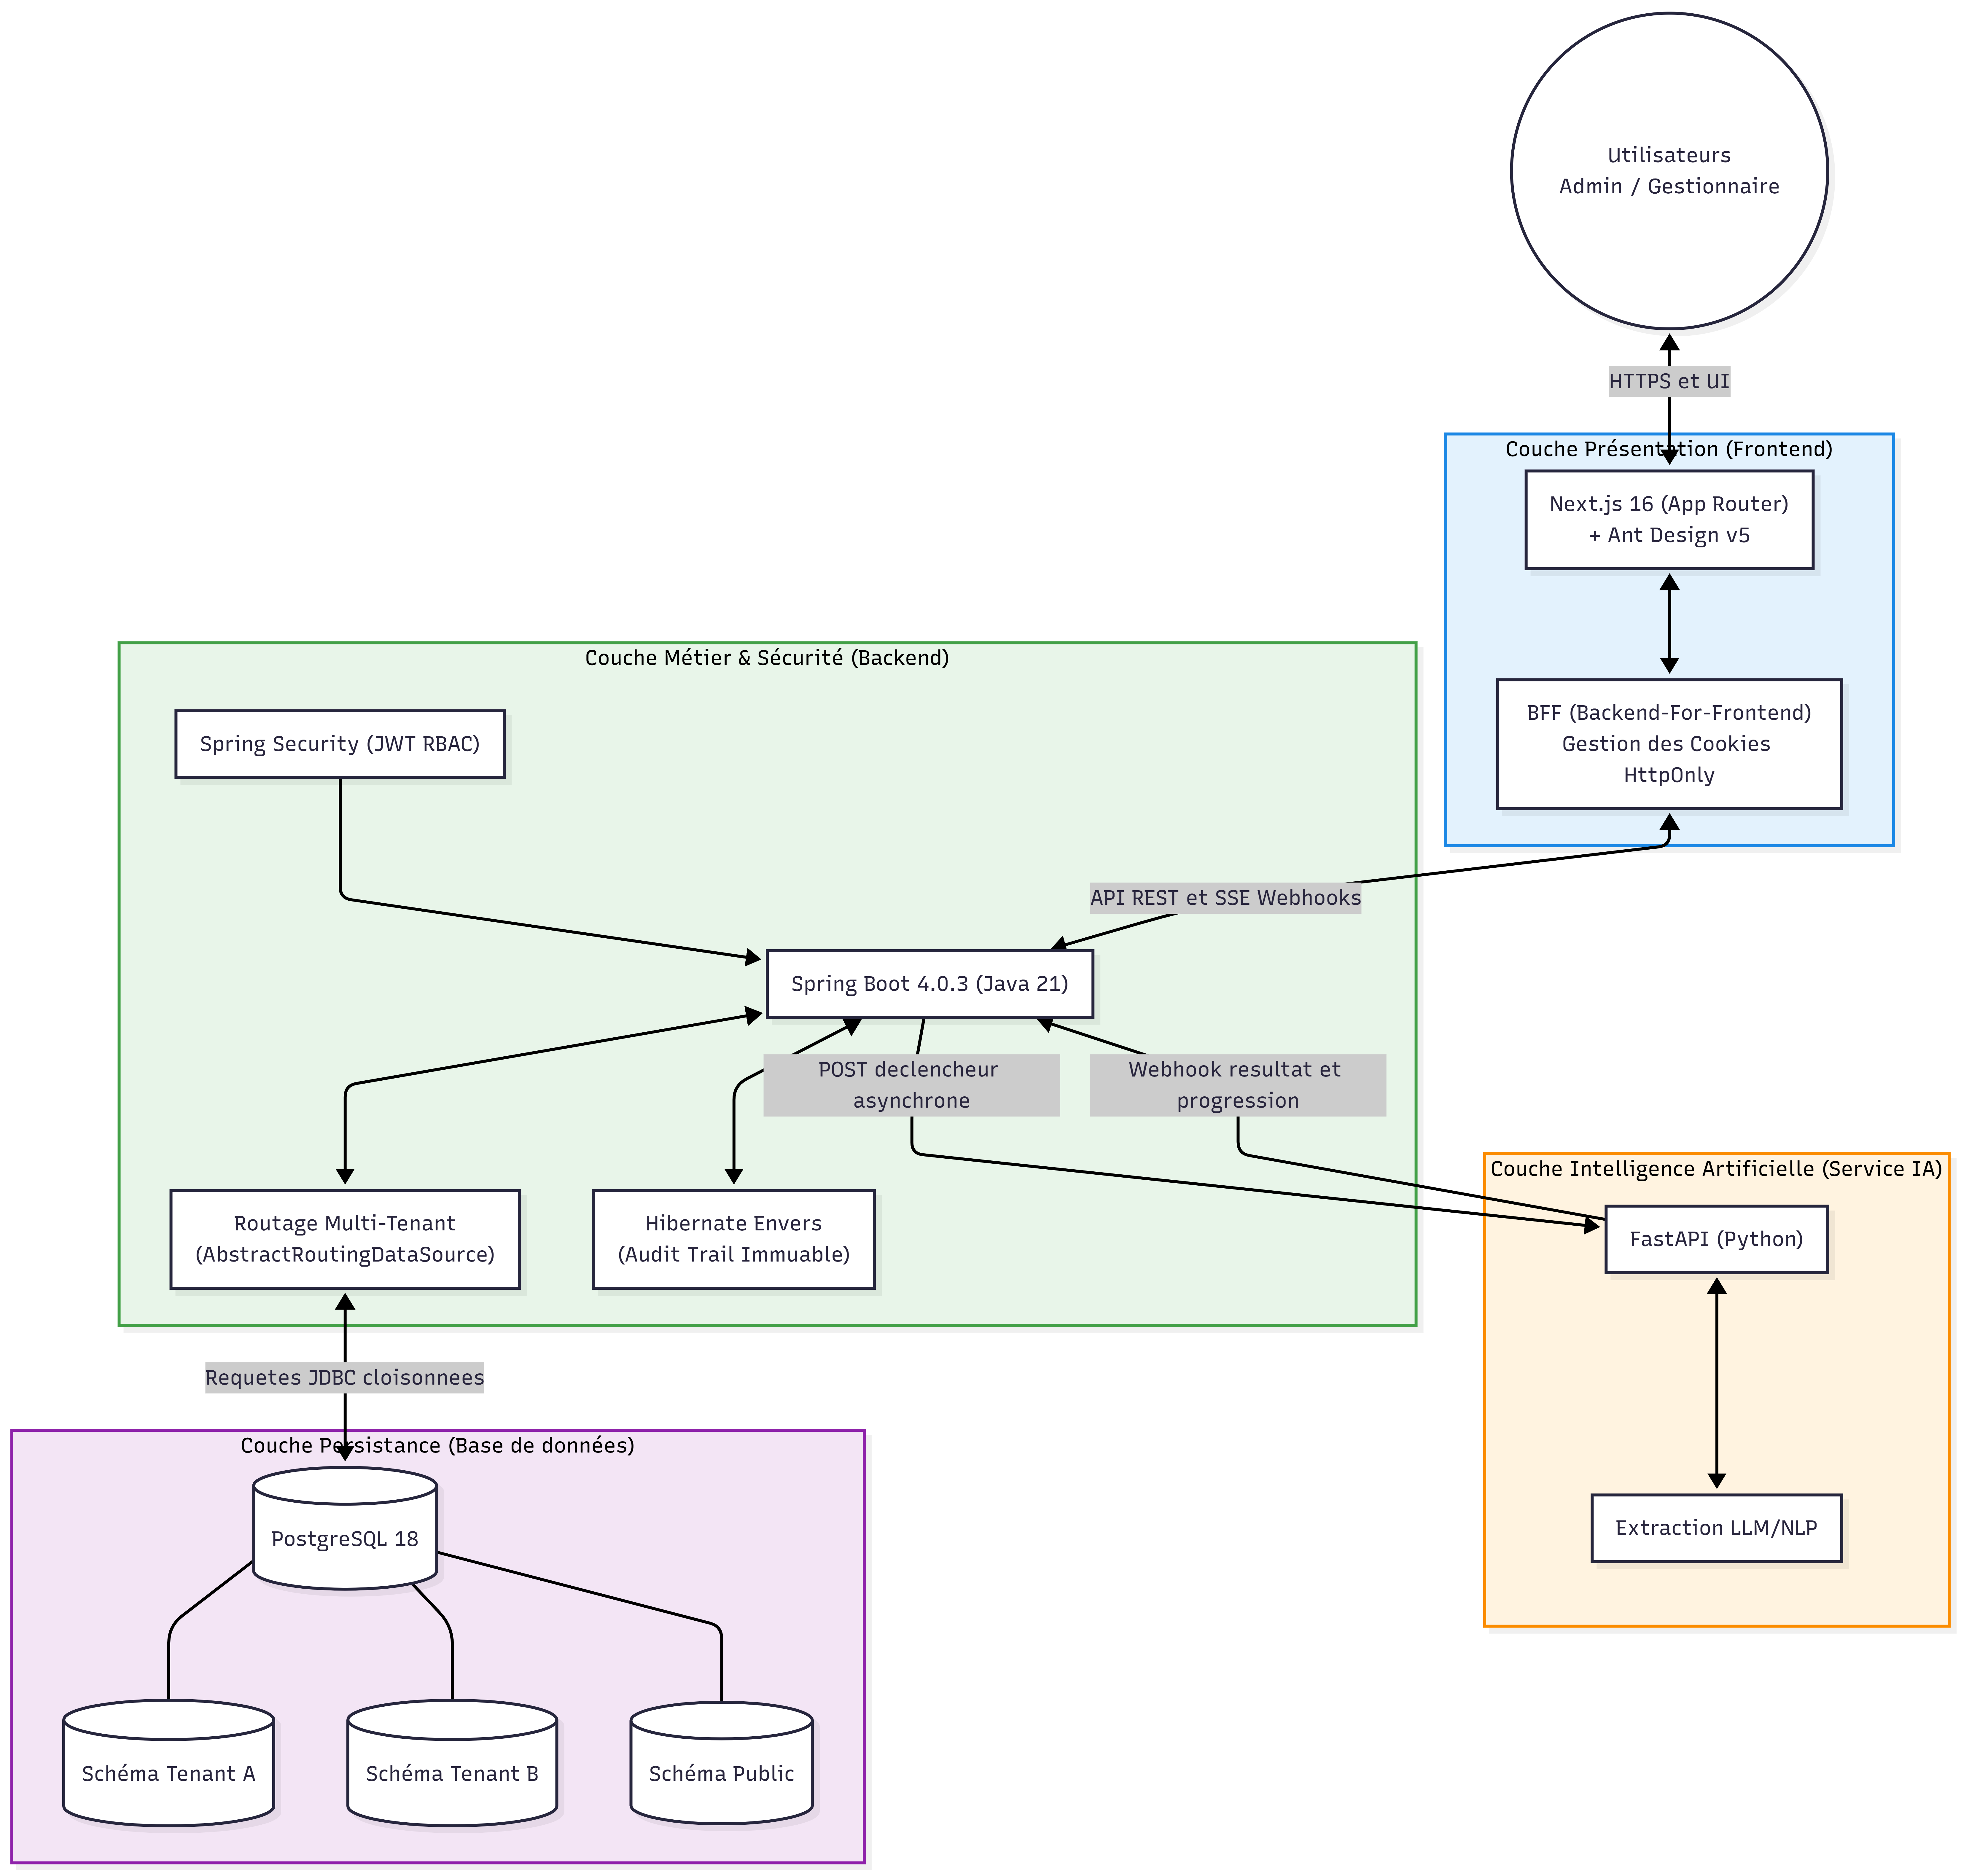
\includegraphics[width=1\textwidth,keepaspectratio]{images/logic-architecture.png}
\caption{Architecture logique du système LeasRecover}
\label{fig:logic_architecture}
\end{figure}

\begin{enumerate}
    \item \textbf{La Couche Présentation (Frontend -- Next.js 16) :} Interface utilisateur réactive développée avec Next.js 16 et la bibliothèque graphique Ant Design. Elle intègre un pattern \textbf{Backend-For-Frontend (BFF)} qui gère de manière invisible et sécurisée les jetons de session (cookies HttpOnly), protégeant ainsi l'application contre les attaques XSS et CSRF.
    \item \textbf{La Couche Métier et Sécurité (Backend -- Spring Boot 4 / Java 21) :} Cœur de l'application. Cette API REST centralise toutes les règles de gestion (workflows, autorisations RBAC, traçabilité). Elle garantit l'isolation multi-tenant en orientant dynamiquement chaque requête vers le schéma de base de données exclusif de la société cliente.
    \item \textbf{La Couche d'Intelligence Artificielle (Service FastAPI / Python) :} Microservice asynchrone haute performance dédié à l'extraction de données complexes (LLM/NLP). Il ingère les rapports d'expertise, extrait les valeurs financières et transmet ses calculs au Backend sans bloquer l'expérience utilisateur.
\end{enumerate}

\subsection{Architecture Physique et Déploiement}

Le déploiement repose sur une infrastructure moderne entièrement conteneurisée. L'ensemble des services (Next.js, Spring Boot, FastAPI) ainsi que la base de données \textbf{PostgreSQL 18} sont encapsulés et orchestrés via \textbf{Docker Compose}. Cette conteneurisation garantit une reproductibilité parfaite et une isolation stricte entre environnements de développement et de production.

\section{Étude de l'environnement}

\subsection{Environnement Matériel}

Le développement a été réalisé sur un poste de travail standard équipé d'un processeur Intel Core i7 et de 16 Go de mémoire vive (RAM), suffisant pour l'orchestration locale des conteneurs Docker et l'exécution des tests.

\subsection{Environnement Logiciel}

\begin{itemize}
    \item \textbf{Next.js 16 \& Ant Design :} Framework React privilégié pour sa robustesse, son routage moderne et ses composants graphiques riches.
    \item \textbf{Spring Boot 4 (Java 21) :} Framework back-end d'entreprise de référence, offrant des fonctionnalités avancées pour la sécurité et la gestion transactionnelle multi-tenant.
    \item \textbf{FastAPI (Python) :} Framework asynchrone haute performance, idéal pour exposer les pipelines d'IA et exécuter les traitements NLP/LLM intensifs.
    \item \textbf{PostgreSQL 18 :} SGBD relationnel robuste choisi pour sa fiabilité transactionnelle ACID et sa gestion efficace des schémas de données isolés.
    \item \textbf{Docker \& Docker Compose :} Outils de virtualisation légère assurant le déploiement cohérent et reproductible des microservices.
\end{itemize}

\clearpage
\section{Conclusion}

Ce chapitre a formalisé de manière exhaustive les exigences fonctionnelles et techniques du système \projectShortTitle. La définition des acteurs, la modélisation UML (diagrammes de cas d'utilisation par module, diagramme de classes), la planification par sprints et l'architecture Next.js / Spring Boot / FastAPI posent un socle particulièrement solide. Le chapitre suivant aborde la conception architecturale détaillée et la modélisation fine des données.
